\section{Implementação} \label{sec:impl}

\subsection{Teoria: Correlação e Convolução}

    A correlação é uma operação em que os pesos são aplicados na ordem em que aparecem visualmente. Assim, considerando o produto Hadamard ($\bar{\cdot}$),  a correlação ($\circ$) de uma região $R$ da imagem por uma máscara $M$ (de dimensões $N \times N$) será \autocite{ref:corrconv}:

\begin{equation*}
    R \circ M = \sum_{i = 1}^N \sum_{j = 1}^N R_{i,j} M_{i,j} = \sum_{i = 1}^N \sum_{j = 1}^N \left(R \,\bar{\cdot}\, M\right)_{i,j}
\end{equation*}

Portanto, a implementação dessa etapa em NumPy poderia ser:

\begin{minted}{python}
    def correlacao_regiao(R: np.ndarray, M: np.ndarray) -> float:
        return np.sum(R * M)
\end{minted}

Podemos ver isso mais visualmente com o seguinte exemplo de um filtro $3 \times 3$ em uma região genérica.

\begin{equation*}
    \begin{bmatrix}
        a & b & c \\
        d & e & f \\
        g & h & k
    \end{bmatrix} \circ \begin{bmatrix}
        0 & 1 & 0 \\
        2 & 3 & 1 \\
        0 & 0 & 0
    \end{bmatrix}
    = b + 2d + 3e + f
\end{equation*}

Apesar disso, a problema pedia a implementação de uma convolução. Nesse processamento a ordem dos elementos de um dos sinais era percorrido de forma contrária, de modo que os sinais fossem combinados na mesma ordem em que aparecem visualmente. Podemos ver isso na \cref{fig:convolucao-sinal}, onde a reflexão do eixo em $g(-\tau)$ faz com que os primeiros pontos de $g(t)$ sejam combinados antes, isto é, $g(t=1)$ aparece antes de $g(t=4)$ na varredura apresentada nos três últimos gráficos.

Com a mesma região $R$ e máscara $M$ acima, a convolução discreta resulta em \autocite{ref:corrconv}:

\begin{equation*}
    R \ast M = \sum_{i = 1}^N \sum_{j = 1}^N R_{i,j} M_{N-i,N-j} \ne R \circ M
\end{equation*}

Observando o exemplo matricial anterior, teremos o seguinte comportamento.

\begin{equation} \label{eq:corrconv}
    \begin{bmatrix}
        a & b & c \\
        d & e & f \\
        g & h & k
    \end{bmatrix} \ast \begin{bmatrix}
        0 & 1 & 0 \\
        2 & 3 & 1 \\
        0 & 0 & 0
    \end{bmatrix}
    = d + 3e + 2f + h =
    \begin{bmatrix}
        a & b & c \\
        d & e & f \\
        g & h & k
    \end{bmatrix} \circ \begin{bmatrix}
        0 & 0 & 0 \\
        1 & 3 & 2 \\
        0 & 1 & 0
    \end{bmatrix}
\end{equation}

A convolução é comumente usada devido a familiaridade das vastas propriedades dessa operação. Por outro lado, a correlação também aparece em vários processamentos de imagem devido à sua aproximação com a visualização de matrizes.

\begin{figure}[H]
    \centering
    \def\svgwidth{12cm}
    \input{figuras/convolucao-sinal.pdf_tex}

    \caption{Exemplo visual da convolução em sinais unidimensionais contínuos.}
    \label{fig:convolucao-sinal}
\end{figure}


\subsection{Código da Convolução}

    A convolução foi implementada em dois \textit{beckends} distintos, com as funções \pyline{convolve} do SciPy \autocite{ref:ndimage} e \pyline{filter2D} do OpenCV \autocite{ref:cvfilter}. A função dos SciPy realiza uma convolução, como definida matematicamente e foi implementada como no \textref{código}{code:scipy}, ignorando o tratamento das bordas.

\begin{listing}[H]
    \begin{minted}{python}
        import numpy as np
        from scipy import ndimage

        def scipy_convolve(input: Image, kernel: Kernel, borda: ...) -> np.ndarray:
            # mudança para float
            input = input.astype(np.float64)
            # convolução
            output = ndimage.convolve(input, kernel, ...)
            return output
    \end{minted}

    \caption{Convolução com o SciPy, sem o tratamento de bordas.}
    \label{code:scipy}
\end{listing}

A biblioteca OpenCV não tem uma operação de convolução, considerando a definição formal. Assim, a função \pyline{cv2.filter2D} faz realmente uma correlação.

Como podemos ver na \cref{eq:corrconv}, as duas operações são similares, bastando reverter a posição dos elementos de uma das matriz. A máscara normalmente é bem menor em relação à imagem, então ela que foi invertida. No caso do OpenCV, esse tipo de inversão das posições, de $(i, j)$ para $(N-i, N-j)$, pode ser feito pelo \pyline{cv2.flip} \autocite{ref:cvflip}, com o argumento \pyline{flipCode} negativo. A implementação da convolução, nesse caso, ficou como no \textref{código}{code:opencv}.

\begin{listing}[H]
    \begin{minted}{python}
        import numpy as np
        import cv2

        def opencv_convolve(input: Image, kernel: Kernel, borda: ...) -> np.ndarray:
            # flip do kernel para a correlação equivalente
            kernel = cv2.flip(kernel, flipCode=-1)
            # convolução
            output = cv2.filter2D(input, cv2.CV_64F, kernel, ...)
            return output
    \end{minted}

    \caption{Convolução com o OpenCV, sem o tratamento de bordas.}
    \label{code:opencv}
\end{listing}

Para selecionar entre os \textit{backends}, existem dois argumentos opcionais. O \mintinline{bash}{--scipy} garante a execução com a biblioteca SciPy, por mais que já seja o padrão. Podemos então conseguir a mesma imagem da \cref{fig:execucao} com o comando:

\begin{minted}{bash}
    $ python3 main.py imagens/baboon.png h1 h2 --scipy
\end{minted}

Do mesmo modo, o OpenCV pode ser escolhido com o argumento \mintinline{bash}{--opencv}.

\begin{minted}{bash}
    $ python3 main.py imagens/baboon.png h1 h2 --opencv
\end{minted}


\subsection{Tratamento de Bordas}

    \begin{figure}[H]
        \centering
        \begin{figure}[H]
    \centering
    \begin{subfigure}{0.48\textwidth}
        \centering
        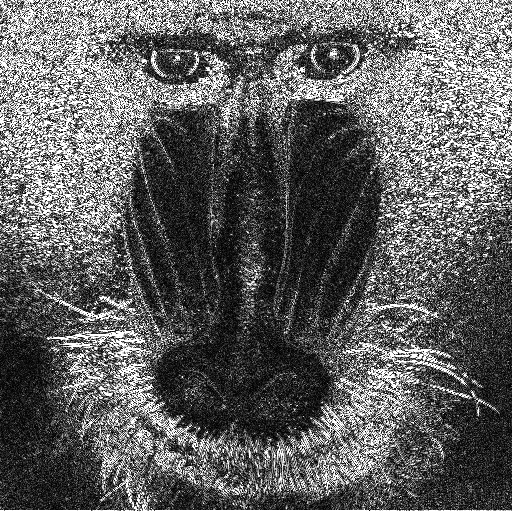
\includegraphics[width=0.9\textwidth]{imagens/baboon.png}
        \caption{Original: \texttt{baboon.png}.}
    \end{subfigure}\\[8pt]
    \begin{subfigure}{0.48\textwidth}
        \centering
        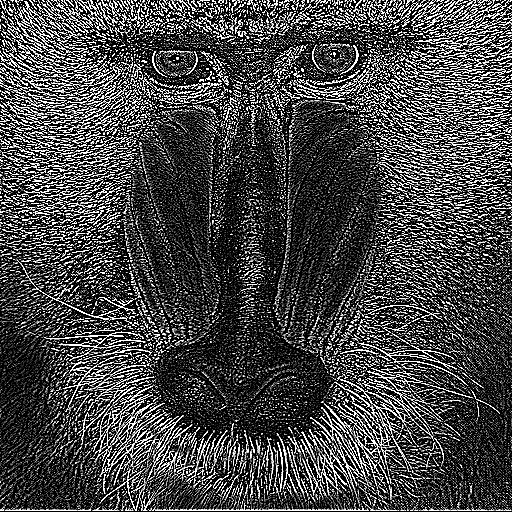
\includegraphics[width=0.9\textwidth]{resultados/baboon_h1.png}
        \caption{Convolução com $h_1$ (\ref{fig:h1}).}
        \label{fig:borda:viz4}
    \end{subfigure}%
    \begin{subfigure}{0.48\textwidth}
        \centering
        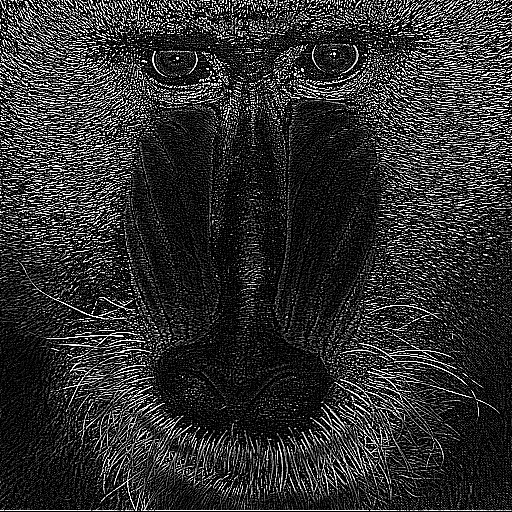
\includegraphics[width=0.9\textwidth]{resultados/baboon_h5.png}
        \caption{Convolução com $h_5$ (\ref{fig:h5}).}
        \label{fig:borda:viz8}
    \end{subfigure}

    \caption{Aplicação do laplaciano discreto.}
\end{figure}

Os filtros de detecção ou realce de bordas mais comuns são os chamados não-direcionais. Normalmente, eles são desenvolvidos a partir do operador laplaciano discreto \autocite{ref:laplacian}. Uma característica importante dos filtros de detecção de bordas é que seus elementos somam zero.

O operador laplaciano serve como uma medida de quanto uma função espacial no ponto $p$ é diferente da média dos pontos em um raio $[p - \delta r, p + \delta r]$. No caso discreto bidimensional, como imagens, existem duas principais medidas de distância, considerando as vizinhaças 4 e 8. Elas resultam em dois tipos de laplacianos diferentes, como pode ser visto na \cref{fig:borda:kernel}.

Nesse trabalho temos o \textit{kernel} $h_1$ (\ref{fig:h1}), com vizinhaça 4 de raio 2, e o $h_5$, com vizinhaça 8 de raio 1. Os resultados podem ser vistos nas figuras \ref{fig:borda:viz4} e \ref{fig:borda:viz8}, respectivamente. Podemos ver que as bordas nas regiões de baixa frequência são bem detectadas, como no centro da imagem, mas regiões de alta frequência resultam em muita informação e podem acabar atrapalhando a análise das bordas. Uma forma de contornar esse problema é aplicando um filtro passa-baixas, como o \textit{blur} gaussiano, discutido na \cref{sec:blur}.

\begin{figure}[H]
    \centering
    \begin{subfigure}{0.4\textwidth}
        \centering
        \begin{kmatrix}
    \matrix[square matrix]{
        0 & 0 & -1 & 0 & 0 \\
        0 & -1 & -2 & -1 & 0 \\
        -1 & -2 & 16 & -2 & -1 \\
        0 & -1 & -2 & -1 & 0 \\
        0 & 0 & -1 & 0 & 0 \\
    };
\end{kmatrix}
        \caption{~$h_1$}
        \label{fig:h1}
    \end{subfigure}%
    \begin{subfigure}{0.4\textwidth}
        \centering
        \begin{kmatrix}
    \matrix[square matrix]{
        -1 & -1 & -1 \\
        -1 & 8 & -1 \\
        -1 & -1 & -1 \\
    };
\end{kmatrix}
        \caption{~$h_5$}
        \label{fig:h5}
    \end{subfigure}

    \caption{Filtros laplacianos discretos}
    \label{fig:borda:kernel}
\end{figure}

A execução pode ser feita com:

\begin{minted}{bash}
    $ python3 main.py imagens/baboon.png h1
    # ou
    $ python3 main.py imagens/baboon.png h5
\end{minted}


        \caption{Argumentos válidos para \mintinline{bash}{--borda} ou \mintinline{bash}{-b}.}
        \label{fig:borda}
    \end{figure}

    Para que a convolução possa ser feita nas bordas da imagem, existem vários modos de tratamento. Na ferramenta foram implementadas três formas de dentre as várias possíveis: a extensão do último pixel (\ref{fig:borda:extensao}), a reflexão dos pixels de borda (\ref{fig:borda:reflexao}) e a mesma reflexão, mas sem repetir o pixel mais externo (\ref{fig:borda:reflexao-pulada}).

    A \textit{flag} \mintinline{bash}{--borda}, ou \mintinline{bash}{-b}, serve para controlar o tratamento de borda. As opções devem ser passadas como aparecem na \cref{fig:borda}. Por padrão, o tratamento é feito como na \cref{fig:borda:reflexao-pulada}, como se fosse a opção \mintinline{bash}{-b reflexao_pula_ultimo}. Ambos \textit{backends}, SciPy e OpenCV, funcionam com os três tipos de bordas.

    Apesar de interessante, e em alguns casos importante, o três tratamentos de bordas não alteram muito no resultado da convolução. A razão disso é que os \textit{kernels} desse trabalho são relativamente pequenos.

\subsection{Discretização}

    Toda o processo de convolução é feito com operações de ponto flutuante, buscando evitar \textit{overflow} e problemas de arredondamento. Então, para que a matriz volte a representar uma imagem, é preciso discretizar os valores, para os níveis 0 a 255.

    A forma mais comum é arrendondando os valores para os inteiros mais próximos no intervalo $[0, 255]$. Dessa forma, os valores negativos se tornam 0 e valores maiores que 255 vão para 255. No código, esse método foi implementado na função \pyline{lib.trunca}. Essa é a opção padrão do programa.

    Uma forma alternativa também foi implementada, baseada no mapeamento linear do menor valor da imagem para 0 e do maior para 255. Na ferramenta em Python, esse método de discretização está implementado na função \pyline{lib.transforma_limites} e pode ser selecionada com a opção \mintinline{bash}{-t} na linha de comando. Essa opção não foi muito utilizada neste relatório.

\subsection{Combinação das Imagens}

    Vários filtros podem ser passados como argumento, como no exemplo da \cref{sec:execucao}. Os filtros são aplicados, um por vez, na mesma imagem de entrada, discretizados e só então combinados em uma imagem final. A combinação é feita pela raiz da soma quadrática, em ponto flutuante, e discretizada novamente.

    Para padronizar a implementação, a etapa de combinação é feita mesmo com apenas uma imagem. Por causa disso, a discretização é feita antes e depois da combinação, mantendo o resultado esperado da convolução. No entanto, isso pode ser alterado com a opção \mintinline{bash}{-n}, fazendo com que a discretização seja aplicada apenas no final.

    Para um filtro apenas, isso faz com que a convolução seja tratada pelo valor absoluto, fazendo as imagens ficarem com regiões mais claras, onde anteriormente seria preto. Esse modo não foi utilizado neste relatório.
